\documentclass{exam}
\usepackage{tikz}
\usepackage{amssymb}
\usepackage{amsmath}
\title{CS113/DISCRETE MATHEMATICS-SPRING 2024}
\author{Worksheet 24}
\date{Topic: Graph Representation and Isomorphism}
\begin{document}
\maketitle
\vspace{5mm}
\begin{center}
\fbox{\fbox{\parbox{5.5in}{\centering In today's session, we'll be exploring a fundamental concept in graph theory known as "Isomorphism." This powerful tool allows us to compare and analyze graphs in a way that preserves their underlying structures, irrespective of how they might appear on the surface. Happy Learning!}}}
\end{center}
\vspace{5mm}

\makebox[0.75\textwidth]{Student's Name and ID:\enspace\hrulefill} 

\vspace{5mm}
\makebox[0.75\textwidth]{Instructor’s name:\enspace\hrulefill}

\vspace{5mm}

\section{Isomorphism:}
The simple graphs \(G_1 = (V_1, E_1)\) and \(G_2 = (V_2, E_2)\) are isomorphic if there exists a one-to-one and onto function \(f\) from \(V_1\) to \(V_2\) with the property that \(a\) and \(b\) are adjacent in \(G_1\) if and only if \(f(a)\) and \(f(b)\) are adjacent in \(G_2\), for all \(a\) and \(b\) in \(V_1\). Such a function \(f\) is called an isomorphism. Two simple graphs that are not isomorphic are called non-isomorphic.

\section{Conditions for Graph Isomorphism:}
Any two graphs will be known as isomorphism if they satisfy the following four conditions:\\
1) There will be an equal number of vertices in the given graphs.\\
\\
2) There will be an equal number of edges in the given graphs.\\
\\
3) There will be an equal amount of degree sequence in the given graphs.\\
\\
4) If the first graph is forming a cycle of length k with the help of vertices {v1, v2, v3, …. vk}, then another graph must also form the same cycle of the same length k with the help of vertices {v1, v2, v3, …. vk}.\\

\section{Important Points:}
1) For any two graphs to be an isomorphism, the necessary conditions are the above-defined four conditions.\\
\\
2) It is not necessary that the above-defined conditions will be sufficient to show that the given graphs are isomorphic.\\
\\
3) If two graphs satisfy the above-defined four conditions, even then, it is not necessary that the graphs will surely isomorphism.\\
\\
4) If the graph fails to satisfy any conditions, then we can say that the graphs are surely not an isomorphism.\\

\vspace{5mm}

\section{Questions}

\begin{questions}

\question
prove or disprove whether the given pair of
graphs is isomorphic. Exhibit an isomorphism or provide a
rigorous argument that none exists. 
\vspace{1in}
\begin{parts}
\part
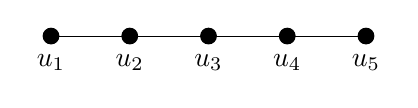
\begin{tikzpicture}
  \node[circle, draw, fill, inner sep=2pt, label=below:$u_1$] (u1) at (0,0) {};
  \node[circle, draw, fill, inner sep=2pt, label=below:$u_2$] (u2) at (1,0) {};
  \node[circle, draw, fill, inner sep=2pt, label=below:$u_3$] (u3) at (2,0) {};
  \node[circle, draw, fill, inner sep=2pt, label=below:$u_4$] (u4) at (3,0) {};
  \node[circle, draw, fill, inner sep=2pt, label=below:$u_5$] (u5) at (4,0) {};
   \draw (0,0) -- (4,0);
\end{tikzpicture}
\vspace{1 in}

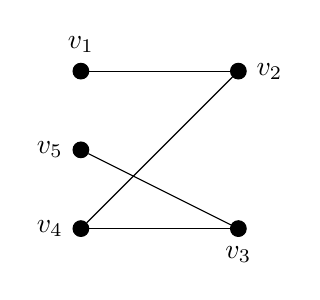
\begin{tikzpicture}
  \node[circle, draw, fill, inner sep=2pt, label=above:$v_1$] (v1) at (0,0) {};
  \node[circle, draw, fill, inner sep=2pt, label=right:$v_2$] (v2) at (2,0) {};
  \node[circle, draw, fill, inner sep=2pt, label=below:$v_3$] (v3) at (2,-2) {};
  \node[circle, draw, fill, inner sep=2pt, label=left:$v_4$] (v4) at (0,-2) {};
  \node[circle, draw, fill, inner sep=2pt, label=left:$v_5$] (v5) at (0,-1) {};

  \draw (v1) -- (v2) ;
  \draw (v4) -- (v2) ;
  \draw (v3) -- (v4) ;
  
  \draw (v3)--(v5);
\end{tikzpicture}
\vspace{3in}

\part
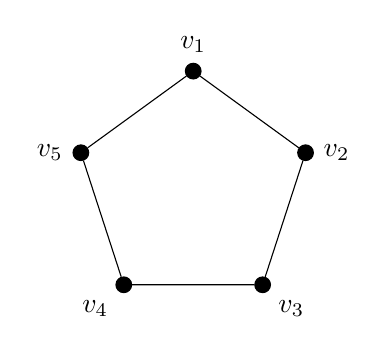
\begin{tikzpicture}
  \node[circle, draw, fill, inner sep=2pt, label=above:$v_1$] (v1) at (90:1.5) {};
  \node[circle, draw, fill, inner sep=2pt, label=right:$v_2$] (v2) at (18:1.5) {};
  \node[circle, draw, fill, inner sep=2pt, label=below right:$v_3$] (v3) at (-54:1.5) {};
  \node[circle, draw, fill, inner sep=2pt, label=below left:$v_4$] (v4) at (234:1.5) {};
  \node[circle, draw, fill, inner sep=2pt, label=left:$v_5$] (v5) at (162:1.5) {};

  \draw (v1) -- (v2) -- (v3) -- (v4) -- (v5) -- (v1);
\end{tikzpicture}

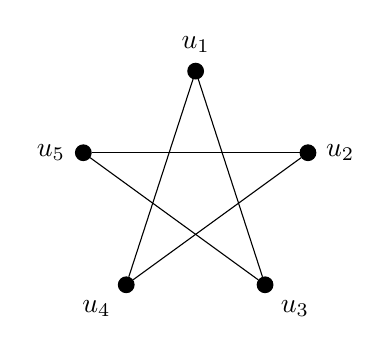
\begin{tikzpicture}
  \node[circle, draw, fill, inner sep=2pt, label=above:$u_1$] (u1) at (90:1.5) {};
  \node[circle, draw, fill, inner sep=2pt, label=right:$u_2$] (u2) at (18:1.5) {};
  \node[circle, draw, fill, inner sep=2pt, label=below right:$u_3$] (u3) at (-54:1.5) {};
  \node[circle, draw, fill, inner sep=2pt, label=below left:$u_4$] (u4) at (234:1.5) {};
  \node[circle, draw, fill, inner sep=2pt, label=left:$u_5$] (u5) at (162:1.5) {};
 
  \draw (u1) -- (u3);
  \draw (u1) -- (u4);
  \draw (u3) -- (u5);
  \draw (u2) -- (u4);
  \draw (u2) -- (u5);
\end{tikzpicture}
\vspace{4in}

\part
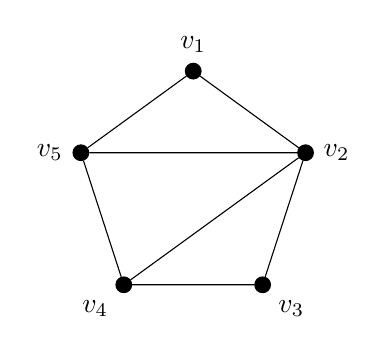
\begin{tikzpicture}
  \node[circle, draw, fill, inner sep=2pt, label=above:$v_1$] (v1) at (90:1.5) {};
  \node[circle, draw, fill, inner sep=2pt, label=right:$v_2$] (v2) at (18:1.5) {};
  \node[circle, draw, fill, inner sep=2pt, label=below right:$v_3$] (v3) at (-54:1.5) {};
  \node[circle, draw, fill, inner sep=2pt, label=below left:$v_4$] (v4) at (234:1.5) {};
  \node[circle, draw, fill, inner sep=2pt, label=left:$v_5$] (v5) at (162:1.5) {};

  \draw (v1) -- (v2) -- (v3) -- (v4) -- (v5) -- (v1);
  \draw (v4) -- (v2) -- (v5);
\end{tikzpicture}

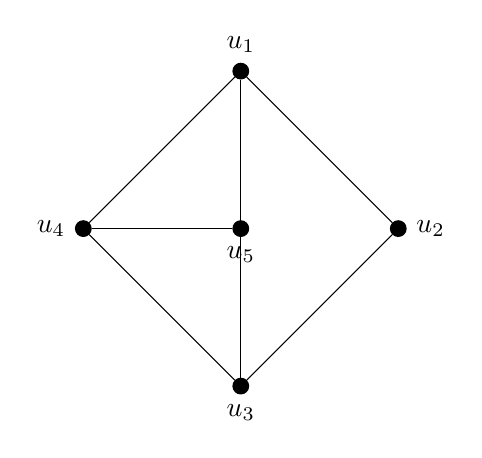
\begin{tikzpicture}
  \node[circle, draw, fill, inner sep=2pt, label=above:$u_1$] (u1) at (0,2) {};
  \node[circle, draw, fill, inner sep=2pt, label=right:$u_2$] (u2) at (2,0) {};
  \node[circle, draw, fill, inner sep=2pt, label=below:$u_3$] (u3) at (0,-2) {};
  \node[circle, draw, fill, inner sep=2pt, label=left:$u_4$] (u4) at (-2,0) {};
  
  \node[circle, draw, fill, inner sep=2pt, label=below:$u_5$] (u5) at (0,0) {};

  \draw (u1) -- (u2) -- (u3) -- (u4) -- (u1);
  \draw (u3) -- (u1);
  \draw (u4)--(u5);
\end{tikzpicture}
\vspace{2in}

\part
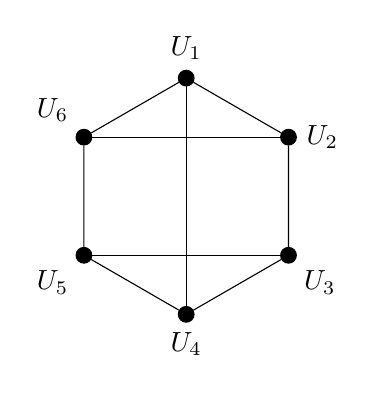
\begin{tikzpicture}
  \node[circle, draw, fill, inner sep=2pt, label=above:$U_1$] (U1) at (90:1.5) {};
  \node[circle, draw, fill, inner sep=2pt, label=right:$U_2$] (U2) at (30:1.5) {};
  \node[circle, draw, fill, inner sep=2pt, label=below right:$U_3$] (U3) at (-30:1.5) {};
  \node[circle, draw, fill, inner sep=2pt, label=below:$U_4$] (U4) at (-90:1.5) {};
  \node[circle, draw, fill, inner sep=2pt, label=below left:$U_5$] (U5) at (-150:1.5) {};
  \node[circle, draw, fill, inner sep=2pt, label=above left:$U_6$] (U6) at (150:1.5) {};

  \draw (U1) -- (U2) -- (U3) -- (U4) -- (U5) -- (U6) -- (U1);
  \draw (U6)--(U2);
  \draw (U5) --(U3);
  \draw (U1) --(U4);
\end{tikzpicture}

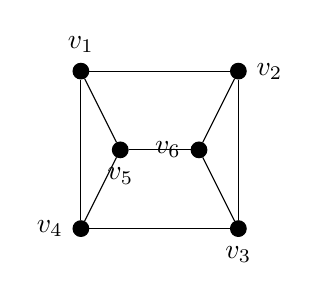
\begin{tikzpicture}
  \node[circle, draw, fill, inner sep=2pt, label=above:$v_1$] (v1) at (0,0) {};
  \node[circle, draw, fill, inner sep=2pt, label=right:$v_2$] (v2) at (2,0) {};
  \node[circle, draw, fill, inner sep=2pt, label=below:$v_3$] (v3) at (2,-2) {};
  \node[circle, draw, fill, inner sep=2pt, label=left:$v_4$] (v4) at (0,-2) {};
   \node[circle, draw, fill, inner sep=2pt, label=below:$v_5$] (v5) at (0.5,-1) {};
  \node[circle, draw, fill, inner sep=2pt, label=left:$v_6$] (v6) at (1.5,-1) {};

  \draw (v1) -- (v2) -- (v3) -- (v4) -- (v1);
  \draw (v1)--(v5)--(v4);
  \draw (v2)--(v6)--(v3);
  \draw (v5)--(v6);
\end{tikzpicture}
\vspace{3in}
\end{parts}
\question 
Suppose that $G$ and $H$ are isomorphic simple graphs. Show that their complementary graphs $\overline{G}$ and $\overline{H}$ are also isomorphic.


\newpage








\end{questions}
\end{document}
